% Drawing 104/01-2 -- folder 104, batch 01, archive page 2 (PDF page 3).
% Transcription: dos d'enveloppe, une vingtaine de figures (complexes cellulaires esquissés) autour des formules. En haut au milieu : un segment à deux extrémités marquées avec une flèche descendante, un segment à trois points, un segment à quatre points, une amande à deux sommets avec une flèche montante. En haut à droite : un petit ovale à un sommet et un ovale à deux sommets, chacun avec une flèche descendante ; au-dessous un disque hachuré coupé par un diamètre et deux amandes hachurées accolées ; puis une sphère avec son équateur, un arc, deux carrés superposés, deux carrés accolés. Au milieu à droite : une bande verticale de trois carrés, une bande horizontale de trois carrés repassée d'un trait épais, un axe gradué de quatre marques partant d'un trait vertical, un carré divisé en quatre aux côtés courbes, un petit segment. En bas : à gauche deux amandes accolées, chacune coupée par son axe ; un quadrillage de trois sur trois, repassé d'un trait épais, avec de petites flèches ; une chaîne de quatre amandes de taille décroissante, chacune coupée par son axe, avec de petites flèches descendantes ; au-dessus une chaîne de quatre flèches horizontales partant du sommet d'une flèche verticale descendante.
% Kind: page of sketched cell complexes: segments, almonds, squares, grids, chains of arrows. Method 2 (schematic redraw from the facsimile). Status: partial.
% Notes: Each figure is redrawn at its place, in a regularised form: segments with their marked points computed on them; almonds as two arcs through the same two tips, consecutive almonds of a chain sharing a tip; strips and grids of squares as rectangles with their dividing lines; the hatched disc and the two hatched almonds with a few hatching strokes; the sphere as a circle with a flat almond for its equator; the two chains of arrows. Left out: all formulas and words (the transcription gives them), the typed address of the envelope, the typescript showing through, the small arrows inside the cells of the 3 by 3 grid and of the chain of four almonds (their directions are not all legible: mostly downwards, some to the right along the top of the grid). Still differs: sizes and positions are read off a wide crop (1 to 2 units); curved sides (the square cut in four, the envelope-shaped almonds) are straightened or smoothed; heavy overdrawing is rendered by one heavy line. Redrawn 2026-11-12 (issue 128): to check again.
% Coordinates: 1 unit = 1 mm = 1/100 of the crop width (bbox in page fractions: [0.17, 0.06, 0.95, 0.5]).
% Redrawn by Claude (claude-fable-5-2), issue #128, 2026-11-12; not checked by a human; not compiled (no TeX in the session).
% Rights: reproduces part of the work -- behind RENDER_TRANSCRIPTS, never published by itself.
\documentclass[tikz,border=3pt]{standalone}
\usepackage{amsmath,amssymb}
\usetikzlibrary{patterns,arrows.meta}
\tikzset{pencil/.style={black!45}, struck/.style={black!35}, mpt/.style={circle,draw,inner sep=1.3pt}, pt/.style={circle,fill,inner sep=0.9pt}, opt/.style={circle,draw,fill=white,inner sep=1.1pt}}
\begin{document}
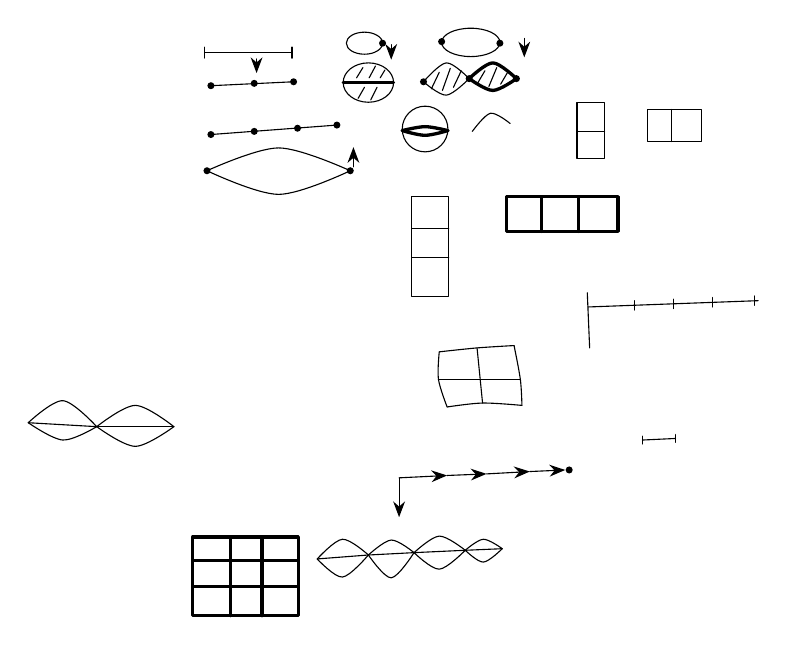
\begin{tikzpicture}[x=1mm,y=1mm,line cap=round,line join=round,font=\scriptsize]
\draw (25.7,-6) -- (36.8,-6);
\draw (25.7,-5.3) -- (25.7,-6.7);
\draw (36.8,-5.3) -- (36.8,-6.7);
\draw[-{Stealth[length=2mm]}] (32.3,-6.8) -- (32.3,-8.6);
\draw (26.5,-10.2) -- (37,-9.7);
\node[pt] at (26.5,-10.2) {};
\node[pt] at (32,-9.9) {};
\node[pt] at (37,-9.7) {};
\draw (26.5,-16.4) -- (42.5,-15.2);
\node[pt] at (26.5,-16.4) {};
\node[pt] at (32,-16) {};
\node[pt] at (37.5,-15.6) {};
\node[pt] at (42.5,-15.2) {};
\draw plot[smooth, tension=0.55] coordinates {(26,-21) (35.1,-18.1) (44.2,-21)};
\draw plot[smooth, tension=0.55] coordinates {(26,-21) (35.1,-24) (44.2,-21)};
\node[pt] at (26,-21) {};
\node[pt] at (44.2,-21) {};
\draw[-{Stealth[length=2mm]}] (44.6,-20.5) -- (44.6,-18);
\draw (46,-4.8) ellipse[x radius=2.3, y radius=1.4];
\node[pt] at (48.3,-4.8) {};
\draw[-{Stealth[length=2mm]}] (49.4,-5) -- (49.4,-6.9);
\draw (46.5,-9.8) ellipse[x radius=3.2, y radius=2.5];
\draw[very thick] (43.3,-9.8) -- (49.7,-9.8);
\draw (45,-9.2) -- (45.8,-7.9);
\draw (46.6,-9.2) -- (47.4,-7.7);
\draw (48,-9.2) -- (48.6,-8.2);
\draw (45.2,-11.8) -- (46,-10.4);
\draw (46.8,-12) -- (47.6,-10.4);
\draw (59.5,-4.7) ellipse[x radius=3.7, y radius=1.8];
\node[pt] at (55.8,-4.6) {};
\node[pt] at (63.2,-4.8) {};
\draw[-{Stealth[length=2mm]}] (66.3,-4.2) -- (66.3,-6.6);
\draw plot[smooth, tension=0.55] coordinates {(53.5,-9.7) (56.4,-7.3) (59.3,-9.3)};
\draw plot[smooth, tension=0.55] coordinates {(53.5,-9.7) (56.4,-11.4) (59.3,-9.3)};
\draw (55.5,-8.5) -- (54.5,-10.6);
\draw (56.9,-8) -- (55.9,-10.8);
\draw (58.3,-8.3) -- (57.3,-10.4);
\draw[very thick] plot[smooth, tension=0.55] coordinates {(59.3,-9.3) (62.3,-7.3) (65.3,-9.3)};
\draw[very thick] plot[smooth, tension=0.55] coordinates {(59.3,-9.3) (62.3,-10.8) (65.3,-9.3)};
\draw (61.3,-8.3) -- (60.3,-10);
\draw (62.8,-7.9) -- (61.8,-10.3);
\draw (64.3,-8.3) -- (63.3,-10);
\node[pt] at (53.5,-9.7) {};
\node[pt] at (59.3,-9.3) {};
\node[pt] at (65.3,-9.3) {};
\draw (53.7,-15.7) circle[radius=2.9];
\draw[very thick] plot[smooth, tension=0.55] coordinates {(50.8,-15.9) (53.7,-15.4) (56.6,-15.9)};
\draw[very thick] plot[smooth, tension=0.55] coordinates {(50.8,-15.9) (53.7,-16.5) (56.6,-15.9)};
\draw plot[smooth, tension=0.55] coordinates {(59.7,-16) (62,-13.7) (64.5,-15)};
\draw (73,-12.3) -- (76.5,-12.3) -- (76.5,-19.5) -- (73,-19.5) -- cycle;
\draw (73,-16) -- (76.5,-16);
\draw (82,-13.2) -- (88.8,-13.2) -- (88.8,-17.3) -- (82,-17.3) -- cycle;
\draw (85,-13.2) -- (85,-17.3);
\draw (52,-24.3) -- (56.7,-24.3) -- (56.7,-37) -- (52,-37) -- cycle;
\draw (52,-28.3) -- (56.7,-28.3);
\draw (52,-32) -- (56.7,-32);
\draw[very thick] (64,-24.3) -- (78.2,-24.3) -- (78.2,-28.7) -- (64,-28.7) -- cycle;
\draw[very thick] (68.5,-24.3) -- (68.5,-28.7);
\draw[very thick] (73.2,-24.3) -- (73.2,-28.7);
\draw (74.3,-36.5) -- (74.6,-43.5);
\draw (74.4,-38.3) -- (96,-37.5);
\draw (80.3,-37.5) -- (80.3,-38.7);
\draw (85.2,-37.3) -- (85.2,-38.5);
\draw (90.2,-37.1) -- (90.2,-38.3);
\draw (95.5,-36.9) -- (95.5,-38.1);
\draw plot[smooth, tension=0.55] coordinates {(55.5,-44) (60.3,-43.5) (65,-43.2)};
\draw plot[smooth, tension=0.55] coordinates {(65,-43.2) (65.8,-47.5) (66,-50.8)};
\draw plot[smooth, tension=0.55] coordinates {(66,-50.8) (61,-50.5) (56.5,-51)};
\draw plot[smooth, tension=0.55] coordinates {(56.5,-51) (55.4,-47.5) (55.5,-44)};
\draw (60.3,-43.5) -- (61,-50.5);
\draw (55.4,-47.5) -- (65.8,-47.5);
\draw (81.3,-55.2) -- (85.5,-55);
\draw (81.3,-54.7) -- (81.3,-55.7);
\draw (85.5,-54.5) -- (85.5,-55.5);
\draw[-{Stealth[length=2mm]}] (50.4,-60) -- (50.4,-65);
\draw[-{Stealth[length=2mm]}] (50.4,-60) -- (56.5,-59.7);
\draw[-{Stealth[length=2mm]}] (56.5,-59.7) -- (61.5,-59.5);
\draw[-{Stealth[length=2mm]}] (61.5,-59.5) -- (67,-59.2);
\draw[-{Stealth[length=2mm]}] (67,-59.2) -- (71.5,-59);
\node[pt] at (72,-59) {};
\draw plot[smooth, tension=0.55] coordinates {(3.3,-53) (7.7,-50.2) (12,-53.5)};
\draw plot[smooth, tension=0.55] coordinates {(3.3,-53) (7.7,-55.2) (12,-53.5)};
\draw (3.3,-53) -- (12,-53.5);
\draw plot[smooth, tension=0.55] coordinates {(12,-53.5) (16.9,-50.8) (21.8,-53.5)};
\draw plot[smooth, tension=0.55] coordinates {(12,-53.5) (16.9,-56) (21.8,-53.5)};
\draw (12,-53.5) -- (21.8,-53.5);
\draw[very thick] (24.2,-67.5) -- (37.6,-67.5) -- (37.6,-77.5) -- (24.2,-77.5) -- cycle;
\draw[very thick] (29,-67.5) -- (29,-77.5);
\draw[very thick] (33,-67.5) -- (33,-77.5);
\draw[very thick] (24.2,-70.5) -- (37.6,-70.5);
\draw[very thick] (24.2,-73.8) -- (37.6,-73.8);
\draw plot[smooth, tension=0.55] coordinates {(40,-70.3) (43.2,-67.8) (46.5,-69.8)};
\draw plot[smooth, tension=0.55] coordinates {(40,-70.3) (43.2,-72.6) (46.5,-69.8)};
\draw (40,-70.3) -- (46.5,-69.8);
\draw plot[smooth, tension=0.55] coordinates {(46.5,-69.8) (49.4,-67.9) (52.3,-69.5)};
\draw plot[smooth, tension=0.55] coordinates {(46.5,-69.8) (49.4,-72.7) (52.3,-69.5)};
\draw (46.5,-69.8) -- (52.3,-69.5);
\draw plot[smooth, tension=0.55] coordinates {(52.3,-69.5) (55.5,-67.4) (58.8,-69.2)};
\draw plot[smooth, tension=0.55] coordinates {(52.3,-69.5) (55.5,-71.6) (58.8,-69.2)};
\draw (52.3,-69.5) -- (58.8,-69.2);
\draw plot[smooth, tension=0.55] coordinates {(58.8,-69.2) (61.1,-67.8) (63.5,-69)};
\draw plot[smooth, tension=0.55] coordinates {(58.8,-69.2) (61.1,-70.7) (63.5,-69)};
\draw (58.8,-69.2) -- (63.5,-69);
\end{tikzpicture}
\end{document}
